% Diagramma dell'architettura (Figura fig:architecture del report).
% Sorgente TikZ autonomo: si compila a parte e il report include il PDF.
%   cd doc/figures && latexmk -pdf architettura.tex
% I valori riportati (repliche, PDB, probe, TTL, path) devono restare
% allineati ai manifest in k8s/ e al codice in api/: se cambiano lì,
% vanno aggiornati qui.
% La larghezza naturale (~16 cm) è scelta per stare in \textwidth con una
% riduzione minima: oltre, il testo \scriptsize diventa illeggibile in stampa.
\documentclass[tikz,border=3pt]{standalone}
\usepackage[T1]{fontenc}
\usepackage{lmodern}
\usetikzlibrary{arrows.meta,positioning,fit,backgrounds,calc}

% Il riquadro del cluster sta su un livello SOTTO quello dei gruppi:
% sullo stesso livello il suo riempimento coprirebbe i gruppi disegnati prima.
\pgfdeclarelayer{bottom}
\pgfsetlayers{bottom,background,main}

% Palette: tinte chiare per i riempimenti, una tinta scura per bordo e testo
% di ogni famiglia di componenti. Leggibile anche in stampa in scala di grigi.
\definecolor{edge}{HTML}{3B4252}
\definecolor{muted}{HTML}{5F6672}
\definecolor{clusterbg}{HTML}{F7F8FA}
\definecolor{netfill}{HTML}{E8EEF7}   \definecolor{netline}{HTML}{3A5A8C}
\definecolor{webfill}{HTML}{EAF3EC}   \definecolor{webline}{HTML}{3F7D4E}
\definecolor{apifill}{HTML}{EEF0FA}   \definecolor{apiline}{HTML}{4B55A0}
\definecolor{redfill}{HTML}{FBECEA}   \definecolor{redline}{HTML}{A3402F}
\definecolor{mgofill}{HTML}{EAF4F1}   \definecolor{mgoline}{HTML}{2F7564}
\definecolor{opsfill}{HTML}{F4F1E8}   \definecolor{opsline}{HTML}{7A6A3A}

\tikzset{
  font=\sffamily\footnotesize,
  >={Stealth[length=2.2mm,width=1.6mm]},
  comp/.style={draw=#1line, fill=#1fill, rounded corners=2pt, line width=0.7pt,
               align=center, inner sep=2.5pt},
  group/.style={draw=#1line, rounded corners=4pt, line width=0.8pt,
                fill=#1fill!55, inner sep=5pt},
  title/.style={font=\sffamily\small\bfseries, text=#1line},
  note/.style={font=\sffamily\scriptsize, text=muted, align=left},
  cmd/.style={->, draw=edge, line width=0.8pt},
  evt/.style={->, draw=edge, line width=0.8pt, dash pattern=on 3pt off 2pt},
  lbl/.style={font=\sffamily\scriptsize, fill=clusterbg, inner sep=1.5pt,
              align=center, text=edge},
  row/.style={draw=apiline!60, fill=white, rounded corners=1pt,
              minimum width=3.0cm, minimum height=0.44cm, inner sep=1pt,
              font=\sffamily\scriptsize},
  store/.style={comp=#1, minimum width=1.95cm, minimum height=1.0cm},
  opsarrow/.style={->, draw=opsline, line width=0.7pt},
}

\begin{document}
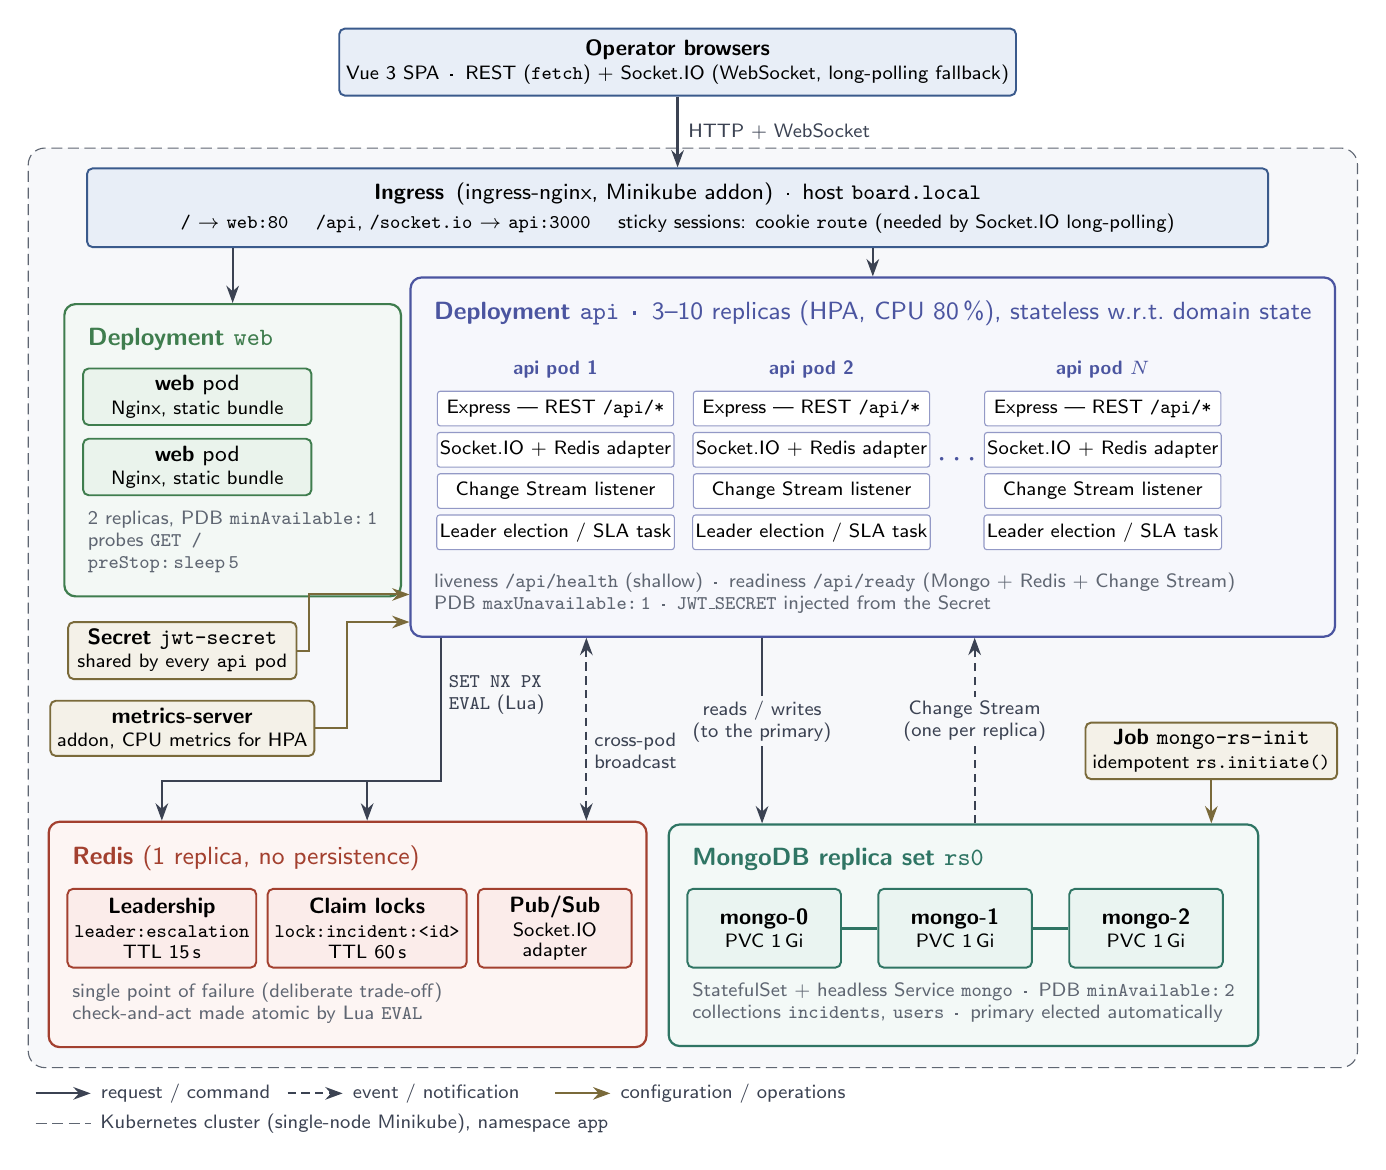
\begin{tikzpicture}

% ---------------------------------------------------------------- client
\node[comp=net, minimum width=8.5cm, minimum height=0.85cm] (browser) at (7.85,13.0)
  {\textbf{Operator browsers}\\[-1pt]
   {\scriptsize Vue~3 SPA \,·\, REST (\texttt{fetch}) + Socket.IO (WebSocket, long-polling fallback)}};

% ---------------------------------------------------------------- ingress
\node[comp=net, minimum width=15.0cm, minimum height=1.0cm] (ingress) at (7.85,11.15)
  {\textbf{Ingress} \,(ingress-nginx, Minikube addon) \,·\, host \texttt{board.local}\\[1pt]
   {\scriptsize \texttt{/} $\to$ \texttt{web:80} \quad
    \texttt{/api}, \texttt{/socket.io} $\to$ \texttt{api:3000} \quad
    sticky sessions: cookie \texttt{route} (needed by Socket.IO long-polling)}};

\draw[cmd] (browser) -- node[lbl, right=2pt, fill=none] {HTTP + WebSocket} (ingress);

% ---------------------------------------------------------------- web
\node[comp=web, minimum width=2.9cm] (web1) at (1.75,8.75) {\textbf{web} pod\\[-1pt]{\scriptsize Nginx, static bundle}};
\node[comp=web, minimum width=2.9cm, below=0.15cm of web1] (web2) {\textbf{web} pod\\[-1pt]{\scriptsize Nginx, static bundle}};
\node[title=web, anchor=south west] (webtitle) at ($(web1.north west)+(-0.05,0.1)$) {Deployment \texttt{web}};
\node[note, anchor=north west] (webnote) at ($(web2.south west)+(-0.05,-0.06)$)
  {2 replicas, PDB \texttt{minAvailable:\,1}\\
   probes \texttt{GET /}\\
   \texttt{preStop:\,sleep\,5}};
\begin{scope}[on background layer]
  \node[group=web, fit=(webtitle)(web1)(web2)(webnote)] (webgrp) {};
\end{scope}

% ---------------------------------------------------------------- api
\newcommand{\apipod}[3]{%
  % #1 nome nodo, #2 x centro, #3 etichetta
  \node[row] (#1r1) at (#2,8.6) {Express --- REST \texttt{/api/*}};
  \node[row, below=0.07cm of #1r1] (#1r2) {Socket.IO + Redis adapter};
  \node[row, below=0.07cm of #1r2] (#1r3) {Change Stream listener};
  \node[row, below=0.07cm of #1r3] (#1r4) {Leader election / SLA task};
  \node[font=\sffamily\scriptsize\bfseries, text=apiline, above=0.03cm of #1r1] (#1t) {#3};
  \begin{scope}[on background layer]
    \node[draw=apiline, fill=apifill, rounded corners=2pt, line width=0.7pt,
          inner sep=2.5pt, fit=(#1t)(#1r1)(#1r4)] (#1) {};
  \end{scope}
}
\apipod{apiA}{6.3}{api pod 1}
\apipod{apiB}{9.55}{api pod 2}
\node[font=\sffamily\bfseries\large, text=apiline] (dots) at (11.4,7.95) {$\cdots$};
\apipod{apiC}{13.25}{api pod $N$}

\node[title=api, anchor=south west] (apititle) at ($(apiA.north west)+(-0.05,0.1)$)
  {Deployment \texttt{api} \,·\, \textmd{3--10 replicas (HPA, CPU 80\,\%), stateless w.r.t.\ domain state}};
\node[note, anchor=north west] (apinote) at ($(apiA.south west)+(-0.05,-0.06)$)
  {liveness \texttt{/api/health} (shallow) \,·\, readiness \texttt{/api/ready} (Mongo + Redis + Change Stream)\\
   PDB \texttt{maxUnavailable:\,1} \,·\, \texttt{JWT\_SECRET} injected from the Secret};
\begin{scope}[on background layer]
  \node[group=api, fit=(apititle)(apiA)(apiC)(apinote)] (apigrp) {};
\end{scope}

\draw[cmd] (ingress.south -| webgrp.north) -- (webgrp.north);
\draw[cmd] (ingress.south -| apigrp.north) -- (apigrp.north);

% ---------------------------------------------------------------- ops (sx)
\node[comp=ops, minimum width=2.9cm, anchor=north west] (secret) at ($(webgrp.south west)+(0.05,-0.3)$)
  {\textbf{Secret} \texttt{jwt-secret}\\[-1pt]{\scriptsize shared by every \texttt{api} pod}};
\node[comp=ops, minimum width=2.9cm, below=0.25cm of secret] (metrics)
  {\textbf{metrics-server}\\[-1pt]{\scriptsize addon, CPU metrics for HPA}};
% Le frecce entrano nel tratto del bordo di api non coperto da web; quella
% di metrics-server sta sotto l'altra, quindi i due percorsi non si incrociano.
\draw[opsarrow] (secret.east) -- ++(0.15,0) |- ($(apigrp.south west)+(0,0.55)$);
\draw[opsarrow] (metrics.east) -- ++(0.4,0) |- ($(apigrp.south west)+(0,0.2)$);

% ---------------------------------------------------------------- redis
\node[store=red] (rlead) at (1.3,2.0)
  {\textbf{Leadership}\\[-1pt]{\scriptsize\texttt{leader:escalation}}\\[-2pt]{\scriptsize TTL 15\,s}};
\node[store=red, right=0.12cm of rlead] (rlock)
  {\textbf{Claim locks}\\[-1pt]{\scriptsize\texttt{lock:incident:<id>}}\\[-2pt]{\scriptsize TTL 60\,s}};
\node[store=red, right=0.12cm of rlock] (rpub)
  {\textbf{Pub/Sub}\\[-1pt]{\scriptsize Socket.IO}\\[-2pt]{\scriptsize adapter}};
\node[title=red, anchor=south west] (redtitle) at ($(rlead.north west)+(-0.05,0.1)$)
  {Redis \textmd{(1 replica, no persistence)}};
\node[note, anchor=north west] (rednote) at ($(rlead.south west)+(-0.05,-0.06)$)
  {single point of failure (deliberate trade-off)\\
   check-and-act made atomic by Lua \texttt{EVAL}};
\begin{scope}[on background layer]
  \node[group=red, fit=(redtitle)(rlead)(rpub)(rednote)] (redgrp) {};
\end{scope}

% ---------------------------------------------------------------- mongo
\node[store=mgo] (m0) at (8.95,2.0) {\textbf{mongo-0}\\[-1pt]{\scriptsize PVC 1\,Gi}};
\node[store=mgo, right=0.45cm of m0] (m1) {\textbf{mongo-1}\\[-1pt]{\scriptsize PVC 1\,Gi}};
\node[store=mgo, right=0.45cm of m1] (m2) {\textbf{mongo-2}\\[-1pt]{\scriptsize PVC 1\,Gi}};
% Replicazione dell'oplog fra i membri (topologia semplificata).
\draw[draw=mgoline, line width=1pt] (m0) -- (m1);
\draw[draw=mgoline, line width=1pt] (m1) -- (m2);
\node[title=mgo, anchor=south west] (mgotitle) at ($(m0.north west)+(-0.05,0.1)$)
  {MongoDB replica set \texttt{rs0}};
\node[note, anchor=north west] (mgonote) at ($(m0.south west)+(-0.05,-0.06)$)
  {StatefulSet + headless Service \texttt{mongo} \,·\, PDB \texttt{minAvailable:\,2}\\
   collections \texttt{incidents}, \texttt{users} \,·\, primary elected automatically};
\begin{scope}[on background layer]
  \node[group=mgo, fit=(mgotitle)(m0)(m2)(mgonote)] (mgogrp) {};
\end{scope}

\node[comp=ops, anchor=south east] (job) at ($(mgogrp.north east)+(1.0,0.55)$)
  {\textbf{Job} \texttt{mongo-rs-init}\\[-1pt]{\scriptsize idempotent \texttt{rs.initiate()}}};
\draw[opsarrow] (job.south) -- (job.south |- mgogrp.north);

% ---------------------------------------------------------------- api <-> data
% Redis. Comandi (claim e leadership) verso le chiavi; pub/sub fra repliche.
\coordinate (rcmd) at ($(apigrp.south west)+(0.4,0)$);
\coordinate (rbus) at ($(rpub.north)+(0.4,0)$);
\coordinate (rfork) at ($(redgrp.north)+(0,0.5)$);
\draw[cmd] (rcmd) |- node[lbl, pos=0.2, right=1pt, align=left] {\texttt{SET NX PX}\\\texttt{EVAL} (Lua)}
  (rfork -| rlead.north) -- (redgrp.north -| rlead.north);
\draw[cmd] (rlock.north |- rfork) -- (redgrp.north -| rlock.north);
\draw[evt, <->] (rbus |- apigrp.south) -- node[lbl, pos=0.62, right=1pt, align=left] {cross-pod\\broadcast} (rbus |- redgrp.north);

% Mongo: scritture/letture verso il primary, change stream verso OGNI replica.
\coordinate (mA) at ($(mgogrp.north west)+(1.2,0)$);
\coordinate (mB) at ($(mgogrp.north west)+(3.9,0)$);
\draw[cmd] (mA |- apigrp.south) -- node[lbl, pos=0.45] {reads / writes\\(to the primary)} (mA);
\draw[evt] (mB) -- node[lbl, pos=0.55] {Change Stream\\(one per replica)} (mB |- apigrp.south);

% ---------------------------------------------------------------- cluster
\begin{pgfonlayer}{bottom}
  \node[draw=muted, dash pattern=on 4pt off 2pt, rounded corners=6pt, fill=clusterbg,
        inner sep=7pt, fit=(ingress)(webgrp)(apigrp)(redgrp)(mgogrp)(job)(metrics)] (cluster) {};
\end{pgfonlayer}

% ---------------------------------------------------------------- legenda
\coordinate (leg) at ($(cluster.south west)+(0.1,-0.32)$);
\draw[cmd] (leg) -- ++(0.7,0) node[right, note, text=edge] {request / command};
\draw[evt] ($(leg)+(3.2,0)$) -- ++(0.7,0) node[right, note, text=edge] {event / notification};
\draw[opsarrow] ($(leg)+(6.6,0)$) -- ++(0.7,0) node[right, note, text=edge] {configuration / operations};
\draw[draw=muted, dash pattern=on 4pt off 2pt] ($(leg)+(0,-0.38)$) -- ++(0.7,0)
  node[right, note, text=edge] {Kubernetes cluster (single-node Minikube), namespace \texttt{app}};

\end{tikzpicture}
\end{document}
